\chapter{Existing solutions} \label{chapter:existing_solutions}
There have been various approaches to design a distributed system that would allow digitising the signals synchronously. Some of them, like OASIS and LIST, are application specific and exist only in one particular laboratory. However, there have been approaches to standardise the way distributed systems should be monitored. The example of such a system is LXI.

For this thesis, it is important to understand these systems and recognise their limitations because the DO as well as the WRTD, which is a crucial tool used to create the DO, are an effort to overcome the limitations of the existing systems.

However, it must be stated, that these systems are crucially different from each other and even though the general goal is the same, each of them serves different purpose. OASIS is meant for monitoring analogue signals, LIST is a trigger distribution system, and LXI is a standard. Therefore this chapter shouldn't be treated as their comparison nor evaluation.

\section{LXI}
    % general description of LXI
    LXI is a specification that standardised the communication protocols for various kinds of laboratory equipment like oscilloscopes, signal generators etc.
    \blockquote[]{
    Key objectives in the development of this standard for test and measurement instrumentation
    include {\cite[8]{specification:LXI}}:
    \begin{enumerate}
        \item Unambiguous communication among LXI Devices
        \item Decreasing the cost of test system software development by the use of industry-standard protocols and interfaces
        \item Provision of a standardised trigger and synchronisation mechanism between LXI Devices
        \item Increasing system performance by using high-speed, Ethernet protocols
        \item Taking advantage of the simplicity of physical Ethernet connectivity.
    \end{enumerate}
    }

    % differentiation of standard and extended functions in order to switch to device synchronisation
    There are two main categories of the LXI standards:
    \begin{itemize}
        \item LXI Device Specification --- These are the rules required by all the LXI conformant devices.
        \item LXI Extended Functions --- This is the set of the optional features.
    \end{itemize}
    
    %Introduction to device synchronisation
    Some of the extended functions refer to device synchronisation and exchanging timestamped events with trigger information. The API for these features is provided in \cite{specification:IVI_LXI_Sync}. The recommended synchronisation method is based on the PTP, described in section \ref{subsec:PTP}. 
    % How does it refer to DO, distributed data acquisition
    Having the means of synchronising the devices and distributing the timestamped events allows implementing various features in the distributed systems:
    \begin{itemize}
        \item synchronisation the events in the system
        \item displaying the signals from distant locations with the known phase relationship
        \item correlation of the data obtained from distant locations
    \end{itemize}
    % what are the drawbacks
    All the described features are desired when creating large systems. However, the frequencies used in modern systems usually are at least in the range of megahertz, while the accuracy of the clock synchronisation in PTP is in the range of microseconds, therefore it is not sufficient. For this reason, there do not seem to be any available devices in the market that implement the LXI Extended Functions for triggers distribution.
    
    The WR network, described in section \ref{section:WR}, extends the PTP, offering sub-nanosecond synchronisation accuracy. WRTD, described in section \ref{section:WRTD}, is designed for exchanging the triggers in distributed systems. It uses the WR for the synchronisation and the data exchange. In order to make it a tool that will be easily integrated with existing systems it implements the LXI Extended Functions for synchronisation and events exchange. WRTD is an essential tool for the project described in this thesis --- the Distributed Oscilloscope.

\section{LIST}
    The LIST project has been deployed as a result of the need for monitoring the LHC instabilities. For that purpose, it was necessary to distribute the triggers between the devices in such a way that when one of them detects the instability, it could synchronously trigger other devices. 
    
    Two timing systems have already been deployed, that were considered to serve the purpose of distributing the triggers:
    \begin{itemize}
        \item General Machine Timing
        \item Beam Synchronous Timing
    \end{itemize}
    However, both of these systems are unidirectional and distribute centrally generated triggers to the equipment. For that reason, it would be impossible to receive and distribute the events between the devices. Therefore, it was decided to deploy another system for distributing the instability events --- the LIST. 
    
    The LIST utilises the WR network described in section \ref{section:WR} for device synchronisation and communication. In order to time-stamp the trigger pulses and reproduce them based on the time-stamps, it uses the TDCs (Time to Digital Converters) and the FDs (Fine Delays), respectively. When one of the devices receives an event, it time-stamps the event and propagates it to the other devices. Since all the devices share the same time reference provided by the WR network, the input to output delay can be  programmed to a fixed value, imposed by the propagation delay of the network. Therefore, all the devices that receive the pulse trigger at the same time with the known time relationship with respect to the device that has produced the trigger. The described operation is depicted in Fig. \ref{fig:list} \cite{LIST_instability_diagnostics}.
    \begin{figure}
    	\centerline{\includegraphics[width=0.9\textwidth]{figures/LIST.pdf}}
    	\caption{The principle of the operation of the LIST}
    	\label{fig:list}
    \end{figure}
    
    The WRTD system, described in section \ref{section:WRTD}, is an evolution of the LIST project. The principle of the operation is very similar. The main differences between the systems are the following:
    \begin{itemize}
        \item LIST is designed for a specific purpose, while WRTD is supposed to be a universal tool. 
        \item They have different APIs.
        \item LIST uses an old version of WR.
    \end{itemize}


\section{OASIS}
    OASIS is a system for acquisition and display of the analogue signals from devices located in the particle accelerators at CERN.
    It consists of 3 tiers \cite{OASIS}:
    \begin{itemize}
        \item Front End Computers --- they control the hardware modules responsible for the digitisation of analogue signals. They are located as close as possible to the signal sources in order to preserve the signal integrity. They provide hardware-independent interfaces for the next layer.
        \item Server --- it is a central unit responsible for processing the data and managing the connections.
        \item Applications --- they provide the Graphical User Interface for displaying the data and modifying the settings of the devices.
    \end{itemize}
    
    In order to monitor the signals in the particle accelerators complex in a synchronous way, all the digitisers need to receive the trigger pulse. The trigger pulses provided via coaxial cables are delivered to each of the digitisers. In order to compensate for the latencies caused by the different cable lengths, delay logic is introduced for each signal path. In practice, the users usually display the data from the devices located close to each other and there is no strong need for the compensation, even if the signals are not very well synchronised.
    The major drawbacks of this system are the following:
    \begin{itemize}
        \item Proper synchronisation is difficult since each path has to be compensated separately. Usually, it is not very accurate.
        \item Coaxial cables parameters, like resistance and capacitance, are sensitive to temperature changes \cite{temp_dep_coax_cables}. 
        \item In large systems, the cost of coaxial cables is very high.
        \item Adding a new digitiser requires laying down another coaxial cable.
        \item It is a CERN specific design, therefore it is almost impossible to use it in another facility.
    \end{itemize}
    
    The majority of drawbacks of OASIS come from the trigger distribution system. In future OASIS will use WRTD for trigger distribution, which should improve the precision and the scalability. The DO serves as a demonstrator of a system similar to OASIS, yet much smaller, which uses WRTD to overcome existing issues. The set of technologies, used to implement the DO is presented in the following chapter.


% \section{System used in LHC --- beam synchronous timing}

